\documentclass[11pt,a4paper,preprint]{aastex}
\usepackage{lscape}
\usepackage{multirow}
\usepackage{rotating}
\usepackage{myaasmacros}
\usepackage{bm}
\usepackage{amsmath}
\usepackage{enumerate}
\usepackage{color}
\usepackage{soul}

\usepackage[linewidth=1pt]{mdframed}
\usepackage[left=3cm,right=3cm,top=3cm,bottom=3.5cm]{geometry}
\newcommand{\low}{\mathrm{low}}
\newcommand{\high}{\mathrm{high}}
\newcommand{\kms}{\mathrm{km}\textrm{ }\mathrm{s}^{-1}}
\newcommand{\kpc}{\mathrm{kpc}}
\newcommand{\Mpc}{\mathrm{Mpc}}
\newcommand{\dd}{\mathrm{d}}
\newcommand{\diag}{\mathop{\mathrm{diag}}}
\newcommand{\udot}{\textrm{ }\dot{}\textrm{ }}
\newcommand{\cc}{(\textrm{c.c.})}
\newcommand{\boxme}[1]{\fbox{\parbox{\textwidth}{#1}}}
\newcommand{\tr}{\mathrm{\mathop{Tr}}}
\newcommand{\lie}{\mathcal{L}}
\definecolor{gray}{RGB}{150,150,150}
\newcommand{\invisible}{\textcolor{gray}}
\setlength{\parindent}{0em}

\newcommand*\colvec[3][]{
    \begin{pmatrix}\ifx\relax#1\relax\else#1\\\fi#2\\#3\end{pmatrix}
}

\newcommand{\bmath}[1]{\ensuremath{\bm{#1}}}
\renewcommand{\vec}[1]{\bmath{#1}}
\newcommand{\tens}[1]{{\bf \sf #1}}
\newcommand{\threej}[6]{{
\left(\begin{array}{ccc} #1 & #3 & #5 \\
 #2 & #4 & #6
\end{array}\right)}}

\newcommand{\D}{\mathcal{D}}

\title{The posterior of a Gaussian subject to $\delta$-function constraints}
\author{Andrew Pontzen}

\begin{document}
\maketitle

Consider a $n$-dimensional Gaussian-distributed data vector $x$, with
mean $\langle \vec{x} \rangle = \vec{x}_0$ and covariance $\langle
(\vec{x}-\vec{x_0})(\vec{x}-\vec{x_0})\rangle = \tens{C}$. The
probabiliy distribution is
\begin{equation}
p(\vec{x}) \propto \exp \left(-\frac{1}{2} (\vec{x} -
  \vec{x}_0)^{\top} \tens{C}^{-1} (\vec{x}-\vec{x}_0) \right)\textrm{,}
\end{equation}
where we have not bothered with normalization (which will be neglected
throughout).

Supose we know that $\vec{x}$ satisfies the linear constraint
$\vec{\alpha}_1 \cdot \vec{x} = d_1$. Then we can legitimately ask
what the new probability distribution $p_1$ is. In fact, this will
turn out to be another Gaussian which means that if we have further
constraints we can simply apply them one-by-one starting from the
original unconstrained distribution.

In the cosmological context, we take a discrete version of our space
(we can use the limit $n \to \infty$ later). We will be constraining
on the smoothed density, $\vec{x}_{\mathrm{smooth}} = \tens{S}_i
\vec{x}$, at some point (say $i=1$ in the vector). Then
$\alpha_i^{\alpha} = S_i^{\alpha \beta} \delta_{\beta}^{1}$. However we
will not need the explicit form whatsoever.

Schematically, we have $p_1(\vec{x}) \propto p_0(\vec{x})
\delta(\vec{\alpha}_1 \cdot \vec{x} - d_1)$. The $\delta$ function
can be approximated as a Gaussian whose width $\beta$ we will allow to
tend to zero later:
\begin{equation}
p_1(\vec{x}) \propto \lim_{\beta \to \infty} p(\vec{x}) \exp \left[
  -\frac{\beta}{2} \left( \vec{\alpha}_1 \cdot \vec{x} - d_1 \right)^2 \right]
\end{equation}

We want to combine the two Gaussians. We assume the new distribution
will have mean $\langle \vec{x} \rangle = \vec{x}_1$ for some
$\vec{x}_1$, and so write
\begin{equation}
p(\vec{x}) \propto \exp \left[-\frac{1}{2} (\vec{x} -
  \vec{x}_1)^{\top} \left(\tens{C}^{-1} + \beta \vec{\alpha}_1
    \vec{\alpha}_1^{\top} \right) (\vec{x}-\vec{x}_1) -
  \vec{x}_1^{\top} \left(\tens{C}^{-1} + \beta \alpha_1
    \alpha_1^{\top} \right) \vec{x} +
  \vec{x}_0^{\top}\tens{C}^{-1}\vec{x} + \beta d_1
  \vec{\alpha}_1^{\top} \vec{x}  \right]
\end{equation}
Here we've thrown away a whole load of terms which are zero-order in
$\vec{x}$ since they just change the normalization. We require the
three dangling linear-in-$\vec{x}$ terms to vanish thus determining
$\vec{x}_1$. We will need two things; first a normalization for the $\vec{\alpha}_1$ which conveniently can
be chosen\footnote{unless $\vec{\alpha}_1$ is a null direction of
  $\tens{C}$, but then there would be zero probability of our
  constraint in the original distribution, so that case is already meaningless. } as
\begin{equation}
\vec{\alpha}_1^{\top} \tens{C} \vec{\alpha}_1 = 1\textrm{.}\label{eq:norm}
\end{equation}
Second, we'll need the Sherman-Morris formula,
\begin{equation}
(\tens{C}^{-1} + \beta \vec{\alpha}_1 \vec{\alpha}_1^{\top})^{-1} =\tens{C} - \beta \frac{\tens{C} \vec{\alpha}_1 \vec{\alpha}_1^{\top}
  \tens{C}}{1+\beta \vec{\alpha}_1^{\top} \tens{C} \vec{\alpha}_1}
\simeq \tens{C} \left[ 1-(1-\beta^{-1}) \vec{\alpha}_1
  \vec{\alpha}_1^{\top} \tens{C} \right] \textrm{,}
\end{equation}
where I have used $\beta \gg 1$ and the normalization condition
\eqref{eq:norm}.

Then we have
\begin{equation}
\vec{x}_1 = \vec{x}_0 - \left(1-\beta^{-1}\right) \tens{C}
\vec{\alpha}_1 \vec{\alpha}_1^{\top} \vec{x}_0 + \beta \vec{d}_1
\tens{C} \beta^{-1} \vec{\alpha}_1
\end{equation}
and in the limit $\beta \to \infty$,
\begin{equation}
\vec{x}_1 = \left[1-\tens{C} \vec{\alpha}_1 \vec{\alpha}_1^{\top}
\right] \vec{x}_0 + d_1 \tens{C} \vec{\alpha}_1\textrm{.}\label{eq:x1}
\end{equation}
We'll interpret this formula in a moment but first note that
\begin{equation}
\tens{C}_1 \equiv \left(\tens{C}^{-1} - \beta \alpha_1
  \alpha_1^{\top}\right)^{-1} = \lim_{\beta \to \infty} \tens{C}
\left[1-\frac{\beta \vec{\alpha}_1 \vec{\alpha}_1^{\top}
    \tens{C}}{1+\beta} \right] = \tens{C}
\left[1- \vec{\alpha}_1 \vec{\alpha}_1^{\top}
    \tens{C} \right]\label{eq:C1}
\end{equation}
giving our final updated probability distribution function
\begin{equation}
p(\vec{x}) \propto \exp \left(-\frac{1}{2} (\vec{x} -
  \vec{x}_1)^{\top} \tens{C}_1^{-1} (\vec{x}-\vec{x}_1) \right)\textrm{,}
\end{equation}
with $\vec{x}_1$ and $\tens{C}_1$ given by equation \eqref{eq:x1} and
\eqref{eq:C1} respectively.

The properties of the updated mean and variance are quite
intuitive. The mean ensures that $\vec{\alpha}_1 \cdot \langle \vec{x}
\rangle = d_1$:
\begin{equation}
\vec{\alpha}_1 \cdot \langle \vec{x} \rangle = \vec{\alpha}_1 \cdot
\vec{x}_1 = \vec{\alpha}_1 \cdot \vec{x_0} - \vec{\alpha}_1 \cdot
\vec{x}_0 + d_1 = d_1
\label{eq:newvar}
\end{equation}
where I have used the normalization condition \eqref{eq:norm}.

The covariance ensures that there is no variation along that
direction:
\begin{equation}
0=\langle (\vec{\alpha}_1 \cdot \vec{x}-d_1)^2 \rangle =% \dots =
%\alpha_1^{\top}\tens{C}_1 \alpha_1 -d_1^2 = 0.
\vec{\alpha}_1^{\top}\tens{C}_1 \vec{\alpha}_1 %= 0,
\end{equation}
where we have used \eqref{eq:newvar} in the intermediate steps to cancel all terms which contain $\vec{x}_1$ and $d_1$.

This is a generalized version of Hoffman and Ribak 1991 (ApJ).

To satisfy two constraints, for simplicity on an initially zero-mean
field, start with $\vec{x}_0=0$ and iterate equation \eqref{eq:x1} and
\eqref{eq:C1} twice. The attached program does that and verifies that
the realizations after constraining twice respect both constraints.

If one adds a local density enhancement to a larger scale void, the
void is enhanced in peak depth. This correctly maintains the large scale void at
the same averaged depth.

\begin{center}
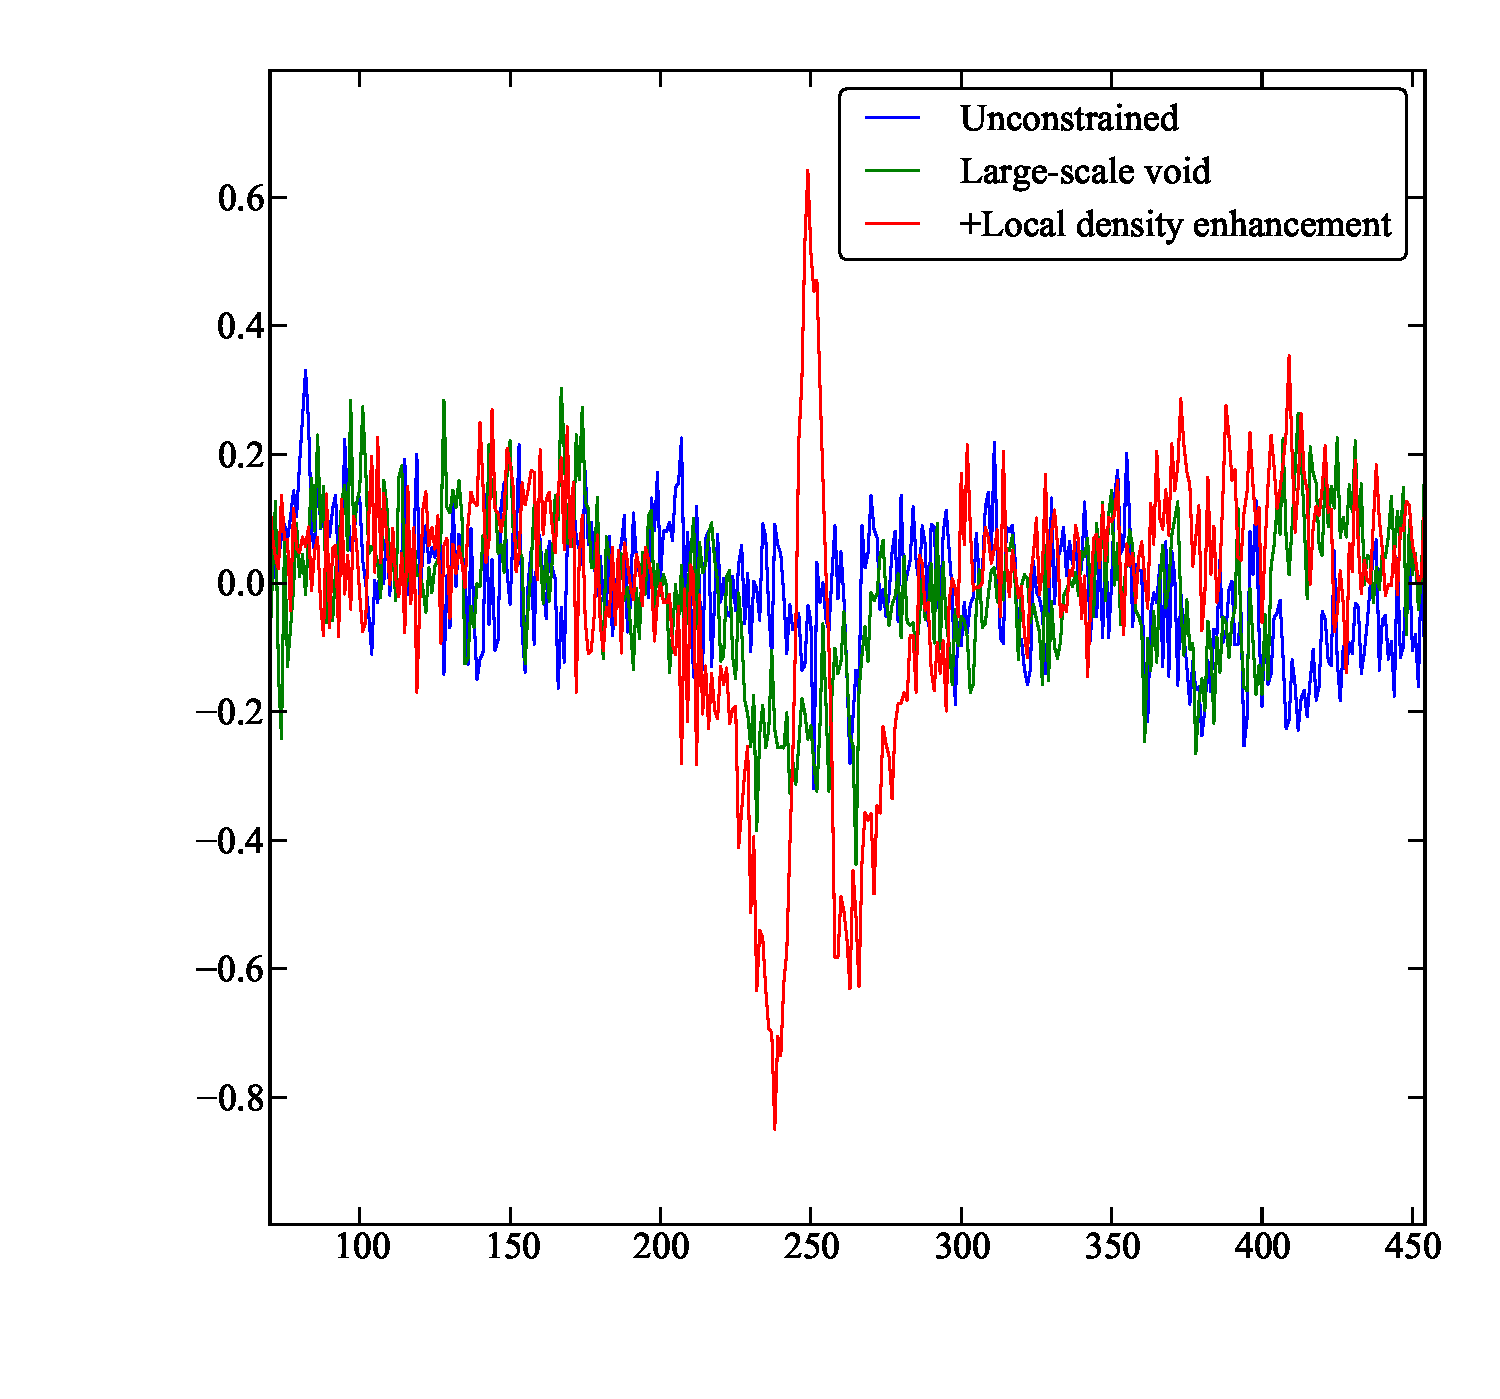
\includegraphics[width=0.5\textwidth]{figs/HR-demo.pdf}
\end{center}


\section{The projection scheme}

Unfortunately the scheme above requires one to sample from the new
covariance matrix $\mathsf{C}_1$. To do that one would need to get the
eigenvalues, and to transform back into a Fourier (or pixel) basis,
also the eigenvectors. This is a horrible problem although Nina made
some progress if we need to go back to it.

Instead if possible let's use an iterative method which works as
follows. The aim is to only ever have diagonal matrices in play. The
strategy is to start with a realization from the original problem --
assumed to be zero mean, covariance $\mathsf{C}$. We can work in
Fourier space so $\mathsf{C}$ is diagonal and multiplication by
$\mathsf{C}$ or $\mathsf{C}^{-1}$ is numerically trivial.

Start by assuming it's possible to get a realization from the
constrained problem by a linear transformation of the unconstrained
problem. Let $\vec{y}_0$ be a realization from the original system and
$\vec{y}_1$ a realization from the constrained system. Then the
assumption is:
\begin{equation}
\vec{y}_1 = (\mathsf{I} + \mathsf{A}) (\vec{y}_0-\vec{x}_0) + \vec{x}_1\textrm{,}\label{eq:y1}
\end{equation}
where by definition $\langle \vec{y}_0 - \vec{x}_0\rangle=0$, so we get the new
mean $\langle \vec{y}_1 \rangle = \vec{x}_1$ which is defined by
equation \eqref{eq:x1}.

Now we can see what condition $\mathsf{A}$ needs to satisfy for us to
get the new covariance correct
\begin{equation}
\langle (\vec{y}_1-\vec{x}_1) (\vec{y}_1-\vec{x}_1)^{\top} \rangle =
\mathsf{C}_1 =
\mathsf{C}_0 - \mathsf{C}_0 \vec{\alpha}_1 \vec{\alpha}_1^{\top} \mathsf{C}_0
\textrm{.}
\end{equation}
using equation \eqref{eq:C1} above.

\subsection{November 2014 - the new scheme}

To solve this, we can just set
\begin{equation}
\mathsf{A} = - \mathsf{C}_0 \alpha_1 \alpha_1^{\dagger}\textrm{,}\label{eq:A}
\end{equation}
which gives
\begin{align}
\mathsf{C}_1 & = (\mathsf{I} - \mathsf{C}_0 \alpha_1
\alpha_1^{\dagger}) \mathsf{C}_0  (\mathsf{I} - \alpha_1
\alpha_1^{\dagger} \mathsf{C}_0 ) \\
& = \mathsf{C}_0 - 2 \mathsf{C}_0 \alpha_1 \alpha_1^{\dagger}
\mathsf{C}_0 + \mathsf{C}_0 \alpha_1 \alpha_1^{\dagger}
\mathsf{C}_0 \alpha_1 \alpha_1^{\dagger}
\mathsf{C}_0  \\
& = \mathsf{C}_0 - \mathsf{C}_0 \alpha_1 \alpha_1^{\dagger}
\mathsf{C}_0\textrm{ as required,}
\end{align}
where I have used the normalization condition \eqref{eq:norm}.

\subsection{For multiple constraints}

The properties of the new field are still Gaussian. So, one can just
recurse. We don't need to know the new covariance matrix explicitly,
thankfully.  As long as one has a routine that can multiply a
$\mathsf{C}_1$ by any arbitrary vector, all is well to calculate with
an arbitrary number of constraints. This seems to work using
\texttt{projection\_constrained} in the python sample code. The
complexity should be linear in the number of constraints.

\subsection{The old iterative scheme}

{\bf Health warning: \it this is actually completely unnecessary -- but is kept here for
  historical information}

 We now make two ansatz, first that
$\mathsf{A} = \mathsf{C}_0 \tilde{\mathsf{A}}$, second that $\mathsf{A} =
\mathsf{A}^{\top}$. [The first can always be made since $\mathsf{C}_0$
is invertible; the second is slightly less clear, but presumably we'd
reach a contradiction if it was invalid? Perhaps this needs a little
thought, but in practice the following works so it must be fine!]

With this transformation, we get the following equation for $\tilde{\mathsf{A}}$:
\begin{equation}
2 \tilde{\mathsf{A}} + \tilde{\mathsf{A}} \mathsf{C}_0
\tilde{\mathsf{A}} = - \vec{\alpha}_1 \vec{\alpha}_1^{\top}
\end{equation}
This is a quadratic equation in the matrix $\tilde{\mathsf{A}}$, which
are generically hard things to solve analytically. However there is an
iterative numerical solution. Namely let us start with the solution
ignoring the quadratic correction,
\begin{equation}
\tilde{\mathsf{A}}_0 = -\frac{1}{2} \vec{\alpha}_1 \vec{\alpha}_1^{\top}\textrm{.}
\end{equation}
(For avoidance of doubt, note the numbering on $\tilde{\mathsf{A}}$ is
not going to count the number of applied constraints like numbering
was earlier on, it's going to count the number of iterations.) Then to
get $\tilde{\mathsf{A}}_{i}$ we apply the formula
\begin{equation}
\tilde{\mathsf{A}}_{i} = -\frac{1}{2} \left(\tilde{\mathsf{A}}_{i-1}
  \mathsf{C}_0 \tilde{\mathsf{A}}_{i-1} + \vec{\alpha}_1 \vec{\alpha}_1^{\top} \right)\textrm{.}
\end{equation}
As written, there are a whole load of matrix operations that we wanted
to avoid! However, suppose we have an algorithm ${\tt calculateA(i-1,z)}$
that calculates $\tilde{\mathsf{A}}_{i-1} \vec{z}$ for any vector
$\vec{z}$, without calculating the enormous matrix
$\tilde{\mathsf{A}}_i$. Then we can write down the algorithm for ${\tt
  calculateA(i,z)}$ as
\begin{equation}
{\tt calculateA(i,z) = -0.5 \left(calculateA(i-1, C_0 \cdot calculateA(i-1,
  z)) + \vec{\alpha}_1 \vec{\alpha}_1^{\top} \vec{z} \right)}\textrm{.}
\end{equation}
Note this algorithm uses only matrix multiplication by $\mathsf{C}_0$
(which is diagonal) and vector dot products. So it is tractable even
for huge $N$!

Then the actual result we want is
\begin{equation}
\vec{y}_1 = \vec{y}_0 + \mathsf{C}_0 \cdot {\tt
  calculateA}(N_{iter},\vec{y}_0) + \vec{x}_1
\end{equation}
where $N_{iter}$ is the total number of iterations. The computational
complexity scales as $N_{iter}^2$, because of the nested calls to {\tt
  calculateA}. But the memory requirements are constant with
$N_{iter}$ (and, when implemented correctly, scale only with the
number of particles, since one never has to store a matrix). I find
$N_{iter}=5$ is plenty for simple 1D test problems.

A demo is provided as {\tt demo2} in the attached program. Here, I
constrain the spatial average value in some region (much like for the
original demo of the basic H-R procedure). The top panels show the
output covariance matrices, from left to right these are
\begin{itemize}
\item The actual exact $\mathsf{C}_1$ calculated from equation
  \eqref{eq:C1} (it's tractable for these test problems of course)
\item The estimate of $\mathsf{C}_1$ from 10\,000 direct realisations,
  showing the level of numerical noise (which goes down with sqrt of
  the number of realisations)
\item The estimate of $\mathsf{C}_1$ from 10\,000 realisations
  calculated using the iterative algorithm, with $N_{iter}=5$. It
  looks like the noise here is pretty consistent with that just from
  the realisation noise, as above.
\item The same, with $N_{iter}=0$.
\end{itemize}

The bottom panels show the errors in the covariance matrix
estimates. For $N_{iter}=5$, these are consistent with just coming
from the realisation noise. For $N_{iter}=0$ there are clearly still
systematic errors (unsurprising!) but the point is you don't need too
many iterations to converge to the right answer.

\st{All in all, I'd have to say this is pretty nice
  stuff. Mathematics, eh?} {\bf Health warning -- \it Pride comes before a fall}

\begin{center}
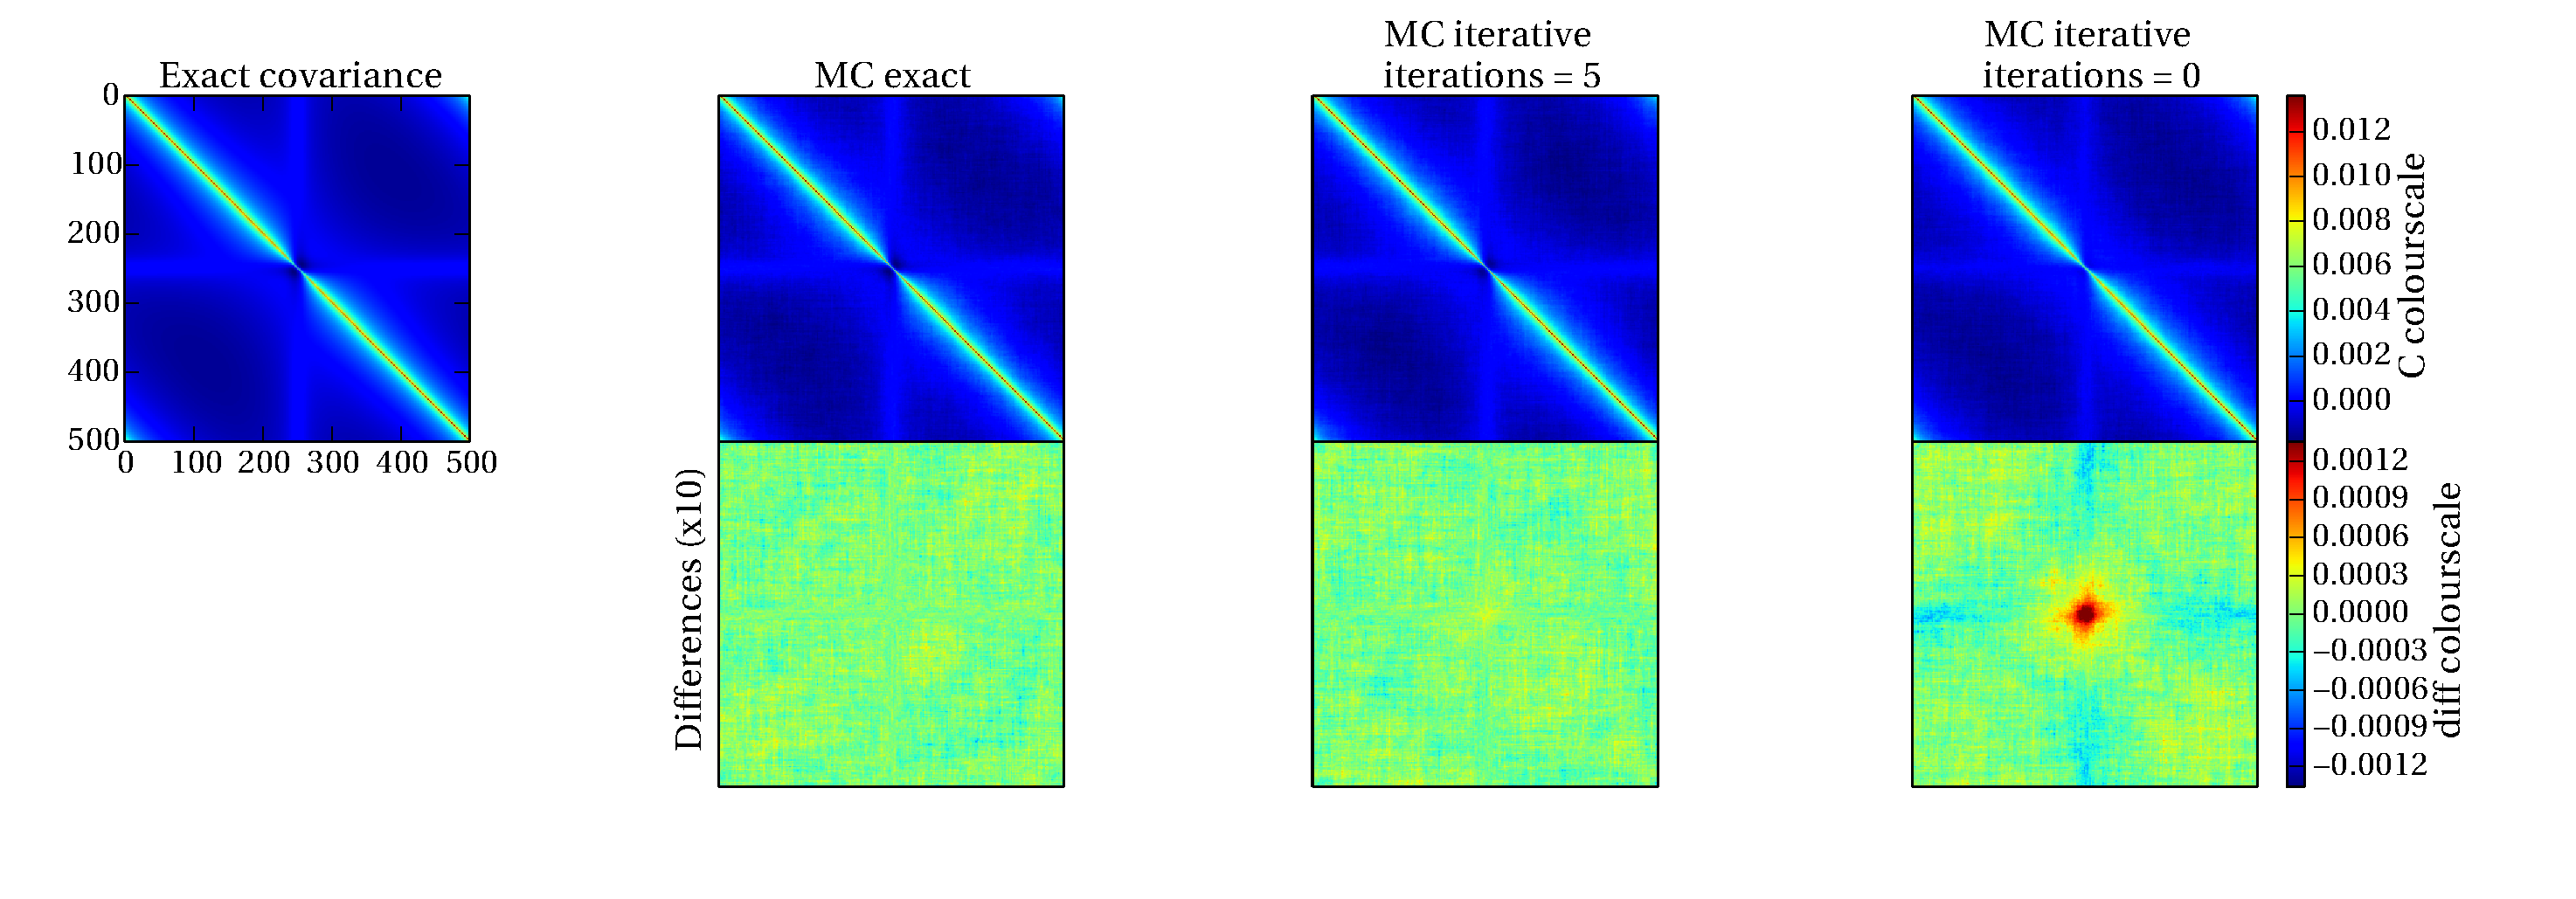
\includegraphics[width=1.1\textwidth]{figs/HR-approx-demo.pdf}
\end{center}

\section{Angular momentum constraints}
\label{sec:AM}

Instead of constraining $\delta$, we actually want to constrain the angular momentum. Fortunately, the method detailed above can be rather straightforwardly extended to do this.

First of all we note that the constraint condition
\begin{equation}
d= \vec{\alpha} \cdot \vec{\delta}
\end{equation}
is equivalent to
\begin{equation}
d= \vec{\alpha}^{\mathrm{P}} \cdot \vec{\phi}
\end{equation}
where $\vec{\delta}$ and $\vec{\phi}$ (the potential) are related via the Poisson equation, and $\vec{\alpha}$ and $\vec{\alpha}^{\mathrm{P}}$ by its inverse.

To linear order, the angular momentum of a set of particles is given by
\begin{equation}
L_{\mu} \propto - \sum_j \sum_{\nu, \rho} \epsilon_{\mu \nu \rho} \vec{x}_j^{\nu} \left[ \partial_{\rho} \vec{\phi} \right] _j
\label{eq:L}
\end{equation}
where Roman indices sum over a set of particles and Greek indices sum over the 3 spatial directions. The final term therefore represents the derivative in direction $\rho$ at position $\vec{x}_j$. We can rewrite this term as a finite difference (here: 4th order)
\begin{equation}
\left[ \partial_{\rho} \vec{\phi} \right] _j =  \partial_{\rho} \phi(\vec{x})|_{\vec{x}=\vec{x}_j} = a \vec{x}_j^{\rho-2} +b\vec{x}_j^{\rho-1} -b \vec{x}_j^{\rho+1} -a \vec{x}_j^{\rho+2}
\end{equation}
where $\vec{x}_j^{\rho+s}$ means the coordinate obtained by shifting of $\vec{x}_j$ by $s$ grid cells in direction $\rho$, $a=1/(12 \Delta) $, $b=-2/(3 \Delta)$, and $\Delta$ is the grid spacing.

If we then require the constrained field to obey
\begin{equation}
L_{\mu} = \vec{\alpha}_{\mu}^{\mathrm{P}} \cdot \vec{\phi},
\label{eq:Lconst}
\end{equation}
we can find the components of $\vec{\alpha}_{\mu}^{\mathrm{P}}$ by comparing terms between the right-hand-sides of equations (\ref{eq:L}) and (\ref{eq:Lconst}). Note that the sum over $j$ in Equation (\ref{eq:L}) can go over an arbitrary number of particles, while the scalar product in Equation (\ref{eq:Lconst}) implies a sum over all grid points. Some components of $\vec{\alpha}^{\mathrm{P}}$ receive contributions from multiple particles, while others may be 0.

After numerically calculating $\vec{\alpha}_{\mu}^{\mathrm{P}}$, we can get the usual $\vec{\alpha}_{\mu}$ from the inverse Poisson equation and iteratively constrain the density field as detailed in the previous section.
One difference here is that there are now technically three constraint
vectors, one for each component of $L_{\mu}$, which are not
independent of each other (in the sense that $\vec{\alpha}_i$ may get
contributions from each direction). Other directions can be
constrained by using linear combinations of these
$\vec{\alpha}_{\mu}$. However, this also means that even if one
chooses a "pure" constraint vector in only one direction, the angular
momentum in the other directions will also change.


\section{Prepare to ZOOM}

To do the really interesting experiments, we need to be able to
prepare zoom initial conditions, i.e. where one has high resolution in
a subregion of the main box. The two really comprehensive references
for how to do this seem to be Bertschinger 2001 (astro-ph/0103301) and
Hahn \& Abel 2011 (1103.6031). Both are written in complex language
that is quite hard to understand.

\subsection{As much as I understand of the existing approaches}

The Bertschinger approach is to generate white noise, using the
Hoffman-Ribak algorithm to constrain the long-wavelength modes in the
high-res subbox to match those of
the low-res superbox. Normally this matching would be very
intensive, requiring a new constraint for every 'pixel' in the low res
box, but because the spectrum is initially completely white, the HR
algorithm becomes trivial (the covariance matrix is just the identity
matrix) and this approach is computationally tractable. However, when
he then applies the transfer function, things become very complicated
because all sorts of artefacts appear on the boundary and must be
avoided using a box of tricks including extending the grid out to
large distances.

Hahn \& Abel use the same observation about the triviality of the HR
algorithm for white noise, but they use a different bag of tricks to
apply the transfer function. They claim this leads to more accurate
results and issue all sorts of obscure warnings for things that can go
wrong.

The trouble is with these approaches for our purposes (beyond their
complexity) is that we need to be able to explicitly calculate
covariances of particular directions in the field. In the
Bertschinger/Hahn+ approach this just doesn't seem to be possible
because the algorithm for constructing the field never makes explicit
what the covarainces between high res and low res elements really
are.

\subsection{But hang on, shouldn't this be easy?}

The weird thing is that I was expecting this part of the problem to be
easy. Naively, you'd think you just lay down a higher res grid in some
subbox, interpolate the low-k modes onto that new grid, then add in
high-k modes to complete the power spectrum in the new region. It's
worth spending a moment to understand why that can't work in practice
as it informs the eventual solution.

If one were to overlay a new high resolution grid completely on top of
the old low resolution grid, the intuition would all work out
fine. Say the new grid has 2x as many points as the old one, then
there are 2x as many Fourier modes. The low Fourier modes match up
exactly, and can be copied across. The high Fourier modes come from a
new realization.  This is then an exact realization on the new
high-resolution grid

The problem comes that the subgrid is not only higher resolution but
also {\it smaller} than the original grid. {\it This means that
  the subbox does not in itself have periodic boundary conditions and
  therefore must have an inhomogeneous correlation function}. This
inhomogeneous correlation function corresponds to a non-trivial
aliasing of power between different Fourier modes coming from the
sharp window function of the high-res region in real space.

To put it another way, most Fourier modes of wavelength $L$ in the
original box will not fit an integer number of times into the subbox
and therefore do not correspond in any simple way to a Fourier mode in the
subbox.

That is why there is no algorithm which simply copies in the low-k
modes and then adds the high-k modes.

\subsection{The multiscale random field without constraints}

Let's split up the problem into the three issues:

\begin{itemize}
\item the resolution split
\item the windowing
\item the pixellization
\end{itemize}

For clarity of notation, we need to be able to express a field in many
different ways.

\begin{itemize}
    \item $\vec{\delta}$ is the real-space vector. In many cases, this only
    exists in a theoretical sense and is too large to realize inside the computer.
    \item $\tilde{\vec{\delta}}$ is the $k$-space vector
    \item $\tilde{\vec{\delta}}^{\low}$ is the $k$-space vector which contains
    only low$-k$ modes.
    \item ${\vec{\delta}}^{\low}$ is the real-space vector one gets from
    inverse fourier transforming the $\tilde{\vec{\delta}}^{\low}$. It is still
    sampled on the same grid of points as the original $\vec{\delta}$ and so still
    can't be fitted inside the computer for our cases of interest
    \item $\vec{\delta}^{\low,P}$ is the re-pixelized vector of low-$k$ modes -- it's
    pixelized at lower resolution
    \item  $\tilde{\vec{\delta}}^{\high}$ is the $k$-space vector which contains
    only high$-k$ modes, such that $\tilde{\vec{\delta}}^{\high}+\tilde{\vec{\delta}}^{\low}=\tilde{\vec{\delta}}$.
    \item $\vec{\delta}^{\high}$ is the inverse fourier transform of $\tilde{\vec{\delta}}^{\high}$
    \item Anything with a $W$ in it is windowed, i.e. is sampled only in the `zoom' region. For example,
    $\vec{\delta}^{\high,W}$ is the windowed, high-$k$ modes. These must be stored on a `fine' grid but
    that's OK as it only exists inside the windowed region.
\end{itemize}

I will try hard to stick to these notations. I don't guarantee it
though since this is a complex document to write and I don't have much
time. If something doesn't make sense it may because I'm being
inconsistent with the notation.

\boxme{{\bf The key point:} We cannot store $\vec{\delta}$, which is
  the overdensity vector across the full box at high
  resolution. However, we can store $\vec{\delta}^{\low,P}$ which is
  the low-resolution vector across the full box sampled at low
  resolution; we can also store $\vec{\delta}^{\high,W}$ which is the
  high-k part of the vector in the subbox; finally, we can also store
  $\vec{\delta}^{W}$ which is the final density field in the subbox.

It sometimes helps to come back to this -- the target of all algorithms is
ultimately to express everything in terms of $^P$ or $^W$ quantities.
The final output consists of the $^{\low,P}$ (unzoomed particles) and the $^{W}$ (zoom particles) vectors.}

The resolution split is relatively straight-forward to deal with in
the absence of windowing and pixelization. We can imagine our final
field $\vec{\delta}$ is made up of two parts with low- and high-
frequencies respectively.  At present we imagine the whole problem is
band-limited and over-pixellized so there are no issues of
pixelization to think of. Then we can just write
\begin{equation}
\vec{\delta} = \vec{\delta}^{\low} + \vec{\delta}^{\high}
\end{equation}

where $\vec{\delta}^{\low}$ and $\vec{\delta}^{\high}$ contain
respectively low and high $k$ modes only. It would be easiest if
there is a particular $k$ scale, $k_0$, where the switch between
fields occurs. However, it turns out this introduces nasty
artefacts when we come to practical implementations later. Basically,
the sharp edges in harmonic space lead to ringing in real space.
So, we have to allow for some $k$ range of overlap between the fields,
with the $\vec{\delta}^{\low}$ tailing off as the $\vec{\delta}^{\high}$ picks
up. Unfortunately this in itself leads to some extra complications,
but they are surmountable. Let's take a look at the first complication.

How would we get a realization of $\tilde{\delta}^{\low}$ and $\tilde{\delta}^{\high}$? There
are two clear possibilities. First, if it's possible to get a realization
of $\tilde{\vec{\delta}}$, we simply need to define
\begin{equation}
  \tilde{\delta}^{\low} = \mathsf{F}^{\low} \tilde{\delta} \hspace{1cm} \tilde{\delta}^{\high} = (1 - \mathsf{F}^{\low}) \tilde{\delta}\label{eq:decompose-delta}
\end{equation}
The sum of $\delta^{\low}$ and $\delta^{\high}$ gives us back
the correct field.

Alternatively, we can start with two independent vectors of white noise
\begin{equation}
\vec{\delta}^R = \tilde{\mathsf{F}}^{\low} \tilde{\mathsf{C}}^{1/2} \tilde{\vec{q}}^{\low} \hspace{1cm} \delta^{\high} = \tilde{\mathsf{F}}^{\high} \tilde{\mathsf{C}}^{1/2} \tilde{\vec{q}}^{\high}\label{eq:gen-low-high}
\end{equation}
where $\tilde{\vec{q}}$ are Gaussian white
noise. This is, for most (but not all) purposes, what we will adopt in practice -- since
we can't actually draw from the full summed field $\tilde{\delta}$ (that's the whole point in the first place).
But what should $\tilde{\mathsf{F}}^{\high}$ be? To check, we need to
get $\tilde{\mathsf{C}}^{\low}$ and $\tilde{\mathsf{C}}^{\high}$:
\begin{equation}
\tilde{\mathsf{C}}^R = \tilde{\mathsf{F}}^R \tilde{\mathsf{C}} \tilde{\mathsf{F}}^{R\dagger}
\end{equation}
where $R=\low$ or $\high$. Then, since $\tilde{\delta} = \tilde{\delta}^{\low} + \tilde{\delta}^{\high}$,
and assuming $\langle \tilde{\delta}^{\low} \tilde{\delta}^{\high}\rangle = 0$ (this is true if we start
from two {\it independent} realizations of noise), we can conclude the filters must satisfy
\begin{equation}
(\tilde{\mathsf{F}}^{\low})^2+ (\tilde{\mathsf{F}}^{\high})^2 = \mathsf{I}\textrm{,}
\end{equation}
to recover the original covariance matrix $\tilde{\mathsf{C}}$ for the full
field. {\bf There is  potential for a lot of confusion here: } unlike method \eqref{eq:decompose-delta},
in equation \eqref{eq:gen-low-high}  the high pass filter
is not one minus the low pass filter. The difference is that in the first case
we were decomposing an existing vector into low and high parts which therefore end
up being correlated, $\langle \tilde{\delta}^{\low} \tilde{\delta}^{\high} \rangle \ne 0$ whereas in the
new case we start off with two separate random noise vectors which therefore are
uncorrelated  $\langle \tilde{\delta}^{\low} \tilde{\delta}^{\high} \rangle = 0$  -- the appropriate
filters are different in these two cases.

{\it Because we use a mixture of these
approaches, it's critical to be very clear about which filter is being
applied at what time.} In both the toy and the production codes, I've used
a Fermi function for $\tilde{\mathsf{F}}^{\low}$,
\begin{equation}
  \tilde{\mathsf{F}}^{\low}_{k_1, k_2}=\frac{\delta_{k_1,k_2}}{1+\exp\left(\frac{k_1-k_{\mathrm{cut}}}{T}\right)}
\end{equation}
where the `temperature' $T$ defines the harshness of the cut-off - I am typically
taking it to be $k_{\mathrm{cut}}/10$ just from playing around.\footnote{In principle
we could do an investigation of what is an optimal trade-off between
suppressing ringing effects and yet keeping the switch-over point well-defined.}

With $\tilde{\mathsf{F}}^{\low}$ fixed, there isn't a unique $\tilde{\mathsf{F}}^{\high}$ because
it depends on which of the above techniques we're using. For the toy code,
{\tt filter\_low} and {\tt filter\_high} implement $\tilde{\mathsf{F}}^{\low}$ and $1-\tilde{\mathsf{F}}^{\low}$
whereas the {\tt C\_filter\_low} and {\tt C\_filter\_high} implement $(\tilde{\mathsf{F}}^{\low})^2$ and $1-(\tilde{\mathsf{F}}^{\low})^2$.
These functions are also named the same in the production code, and can be found in the
{\tt IC} class.

\subsection{Introducing the window and pixelization}

Let's talk about pixelization first. The idea is supposed to be that
the low-pass filter retains $k$ modes that are well sampled even on a
sparse grid. If the window function of the coarse pixels kicks in at
high enough $k$ compared to $k_{\mathrm{cut}}$, we can basically
upsample and downsample between the fine and coarse pixel resolution
without penalty. I experimented with a number of ways of doing this,
but settled on simply linear interpolation to up-sample, and linear
averaging to down-sample. Note that one can cook up much more complex
schemes with apparently desirable properties, but they normally come
with other problems and in practice the only thing that works is to
separate  $k_{\mathrm{cut}}$ and the window scale
sufficiently. Numerical experiments will be shown in Section
\ref{sec:low-res-pixelization}. 

For now, I just want to focus on one source of
confusion/complication. This is the alignment of pixels. Since a pixel
covers a finite volume, what do we mean by the field in 

Now we also have to window the high-resolution part. I am going to switch to
real space to do this.
\begin{align}
\vec{\delta}^{\high,W} & = \mathsf{W} \mathsf{F}^{\high} \mathsf{C}^{1/2}
\vec{q}^{\high}\\
& \equiv \mathsf{WC_{\high}^{1/2}} \vec{q}^{\high} \label{eq:deltaII-ideal}
\end{align}
where $\mathsf{W}$ is the window function which is
diagonal {\it in pixel space} and $\mathsf{C}_{\high}^{1/2} \equiv
\mathsf{F}^{\high} \mathsf{C}^{1/2}$ .  Note in practice, while I'm quite happy to write
things like $\mathsf{W} \mathsf{F}^{\high} \mathsf{C}^{1/2} \vec{q}^{\high}$ to simplify
the equations, the actual
computations involve switching between real and harmonic space, i.e. if you do this in
actual code, you calculate
$\tilde{\mathsf{F}}^{\high} \tilde{\mathsf{C}}^{1/2} \tilde{\vec{q}}^{\high}$ then transform to real space to
do the windowing part.

So far, this could all be done exactly in principle. But we actually need an approximation to replace \eqref{eq:deltaII-ideal}.
Taken literally, eq  \eqref{eq:deltaII-ideal} would involve making a high
resolution data vector covering the entire region, $\vec{q}^{\high}$ ,
which is precisely what computational requirements prevent us from
doing. Instead we want to start from $q^{\high}_W \equiv
\mathsf{W}\vec{q}^{\high}$ -- a shorter, pre-windowed vector that
contains only information from inside the high-res window. In this
case, we actually lack some of the information we technically need,
but we can still do a maximum-likelihood estimate of
$\vec{\delta}^{\high}$, subject to knowing only $\vec{q}^{\high,W}$, which
gives us
\begin{equation}
\vec{\delta}^{\high} = \mathsf{WC_{\high}^{1/2}W}^{\top} (\mathsf{WW}^{\top})^{-1} \vec{q}^{\high,W} \textrm{.}
\end{equation}
Note that $(\mathsf{WW}^{\top})^{-1}$ is just the identity in the
restricted region (it's small x small since $\mathsf{W}$ is small x large).

But we still have a problem! The $\mathsf{WC_{II}^{1/2}W}^{\top}$
cannot be calculated without generating a high-res, full-sized
representation of the covariance matrix. Intuitively, though, we ought
to be able to replace this complicated beast with just the standard
covariance matrix for the appropriate $k$ in the small-scale, high-$k$
limit when the window is basically irrelevant. The question is, how
different is $\mathsf{WC_{II}^{1/2}W}^{\top}$ from $C_{II,W}^{1/2}$
where the latter is just evaluated directly within the window?
At this point, let's switch to numerics to answer the question....


\section{Applying the transfer function -- demos}

Using {\tt constrainedzoom.py} routine {\tt WC\_vs\_CW} here are some
examples of the difference between applying the transfer function
inside the window vs applying it in the full box and windowing
afterwards. All use a power spectrum $P(k) \propto k^{-1}$. Note there
is a significant dependence on the power spectrum. (For white noise,
for example, there is no problem at all because $\mathsf{C}$ is just
the identity matrix.)

Here's what happens if you just naively do the whole problem in the
finite box (4x smaller than the parent domain). The top rows show the
final covariance matrices in real space; the lower rows show the same
in harmonic space. From left to right, we have the ``correct''
solution (which is ultimately intractable); the ``naive'' solution
(just applying $\mathsf{C}$ inside the window); and the error (colour
scale exaggerated by factor 10):

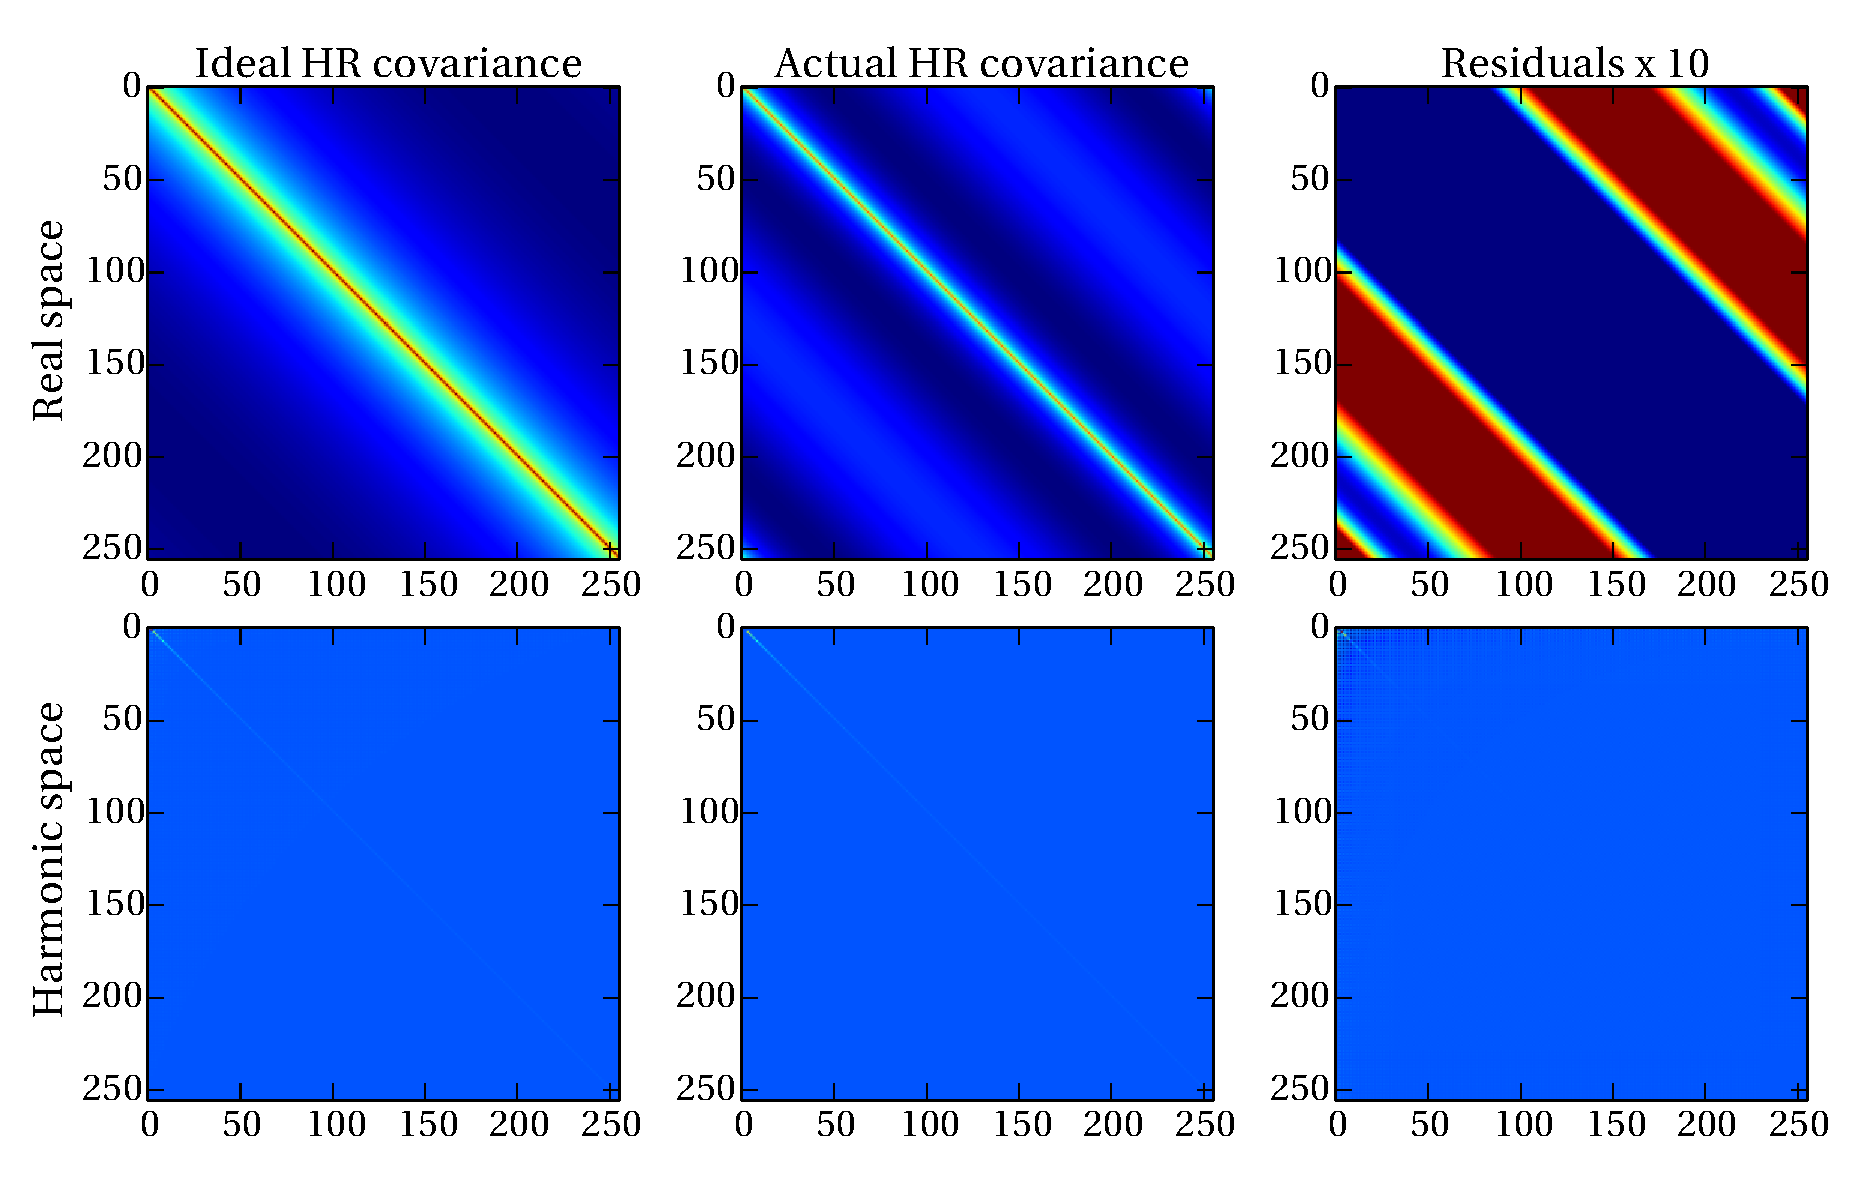
\includegraphics[width=\textwidth]{figs/zoom_test1.pdf}

Note that, in harmonic space, the problems all arise at low $k$ (lower
right panel).
If we cut out all modes with $k/2\pi<0.1L^{-1}$ where $L$ is the
parent box size (and using a Fermi function to soften the cut) we get
this:

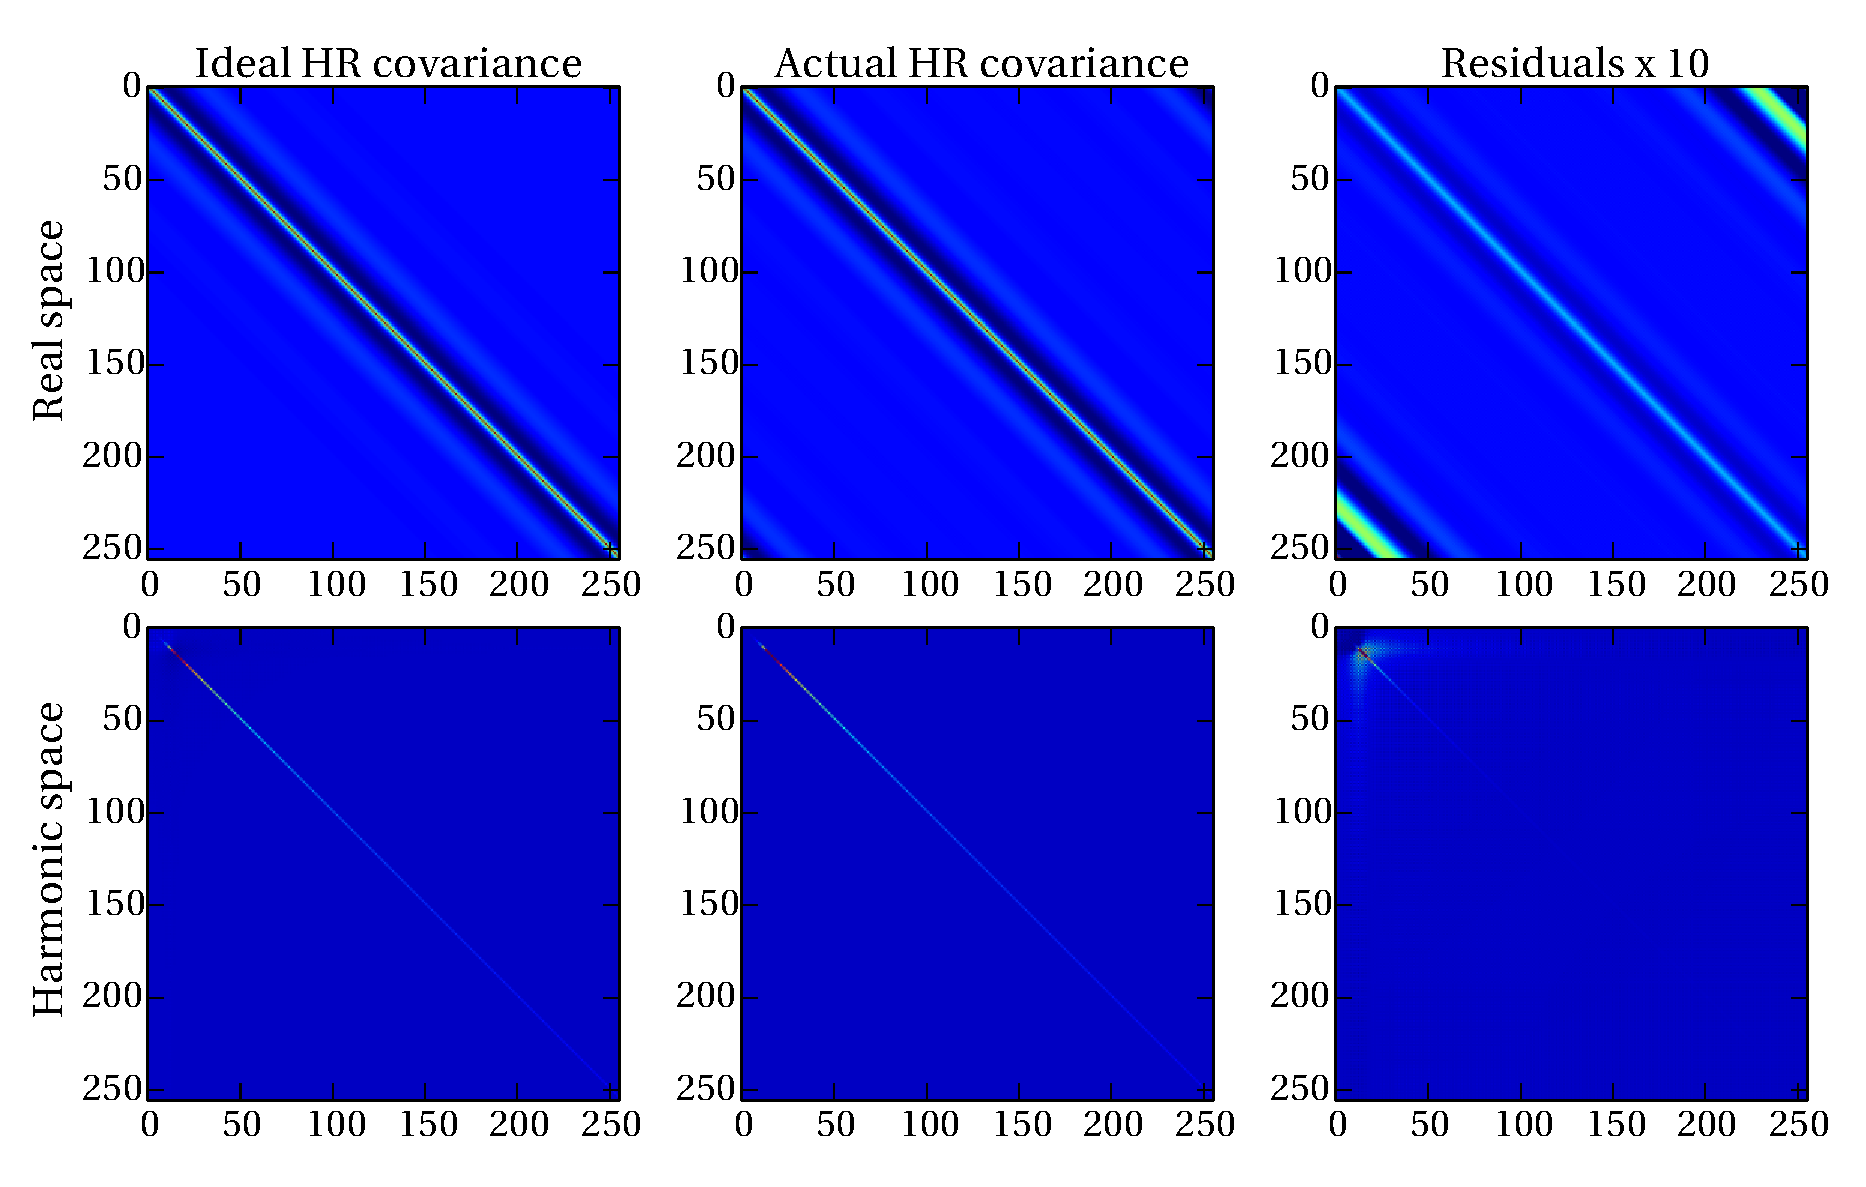
\includegraphics[width=\textwidth]{figs/zoom_test2.pdf}

or at $k/2\pi \le 0.5L$ we get this:

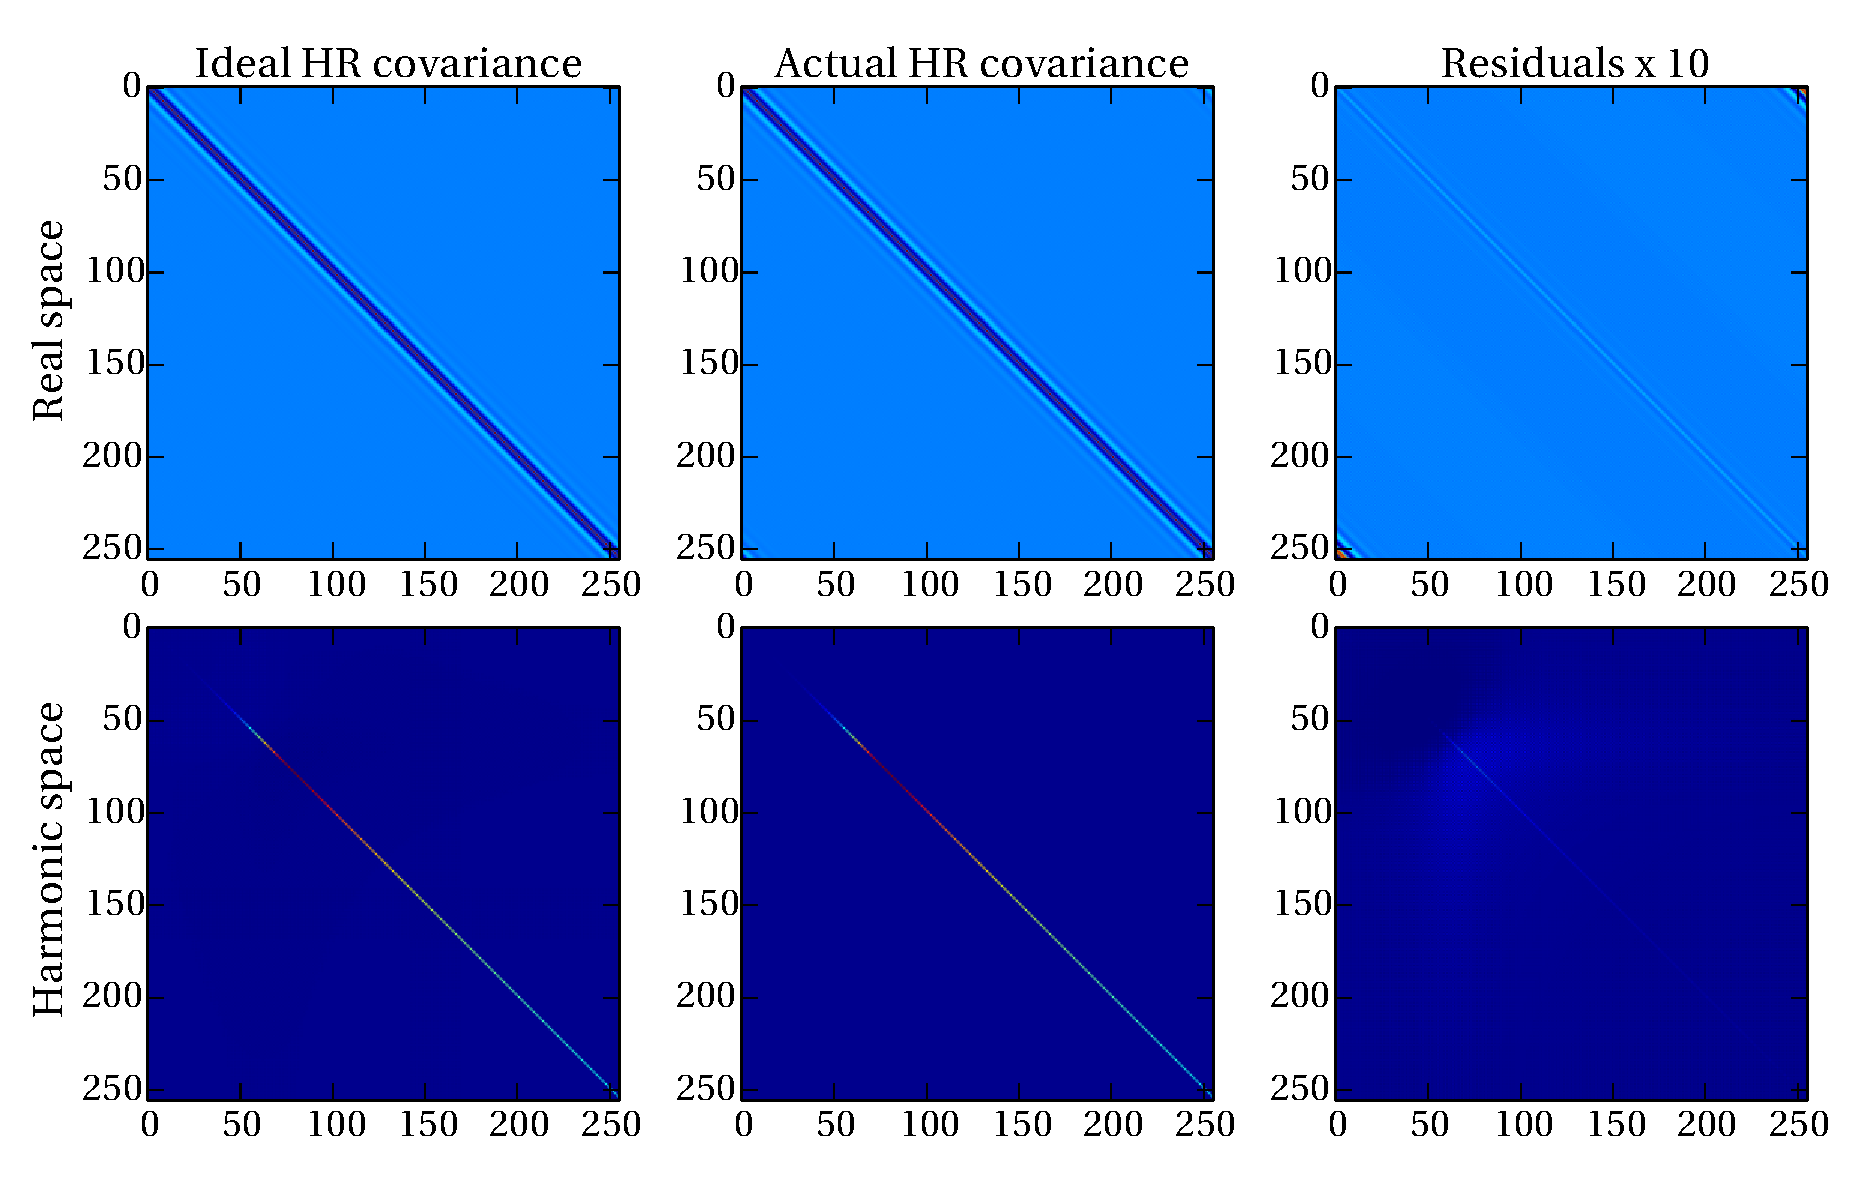
\includegraphics[width=\textwidth]{figs/zoom_test3.pdf}

Things get better as the cut moves to higher $k$. Also things are
typically better closer to the centre of the box rather than at the
edges.  The above were generated using code version {\tt 7806264b}
calling as {\tt cz.WC\_vs\_CW(plaw=-1.0,k\_cut=0.001)}, {\tt
  cz.WC\_vs\_CW(plaw=-1.0,k\_cut=0.1)} and {\tt
  cz.WC\_vs\_CW(plaw=-1.0,k\_cut=0.5)} respectively\footnote{In more recent
  versions, you need to add the keywords {\tt part='hi'}}.

This is a very complex problem, dependent on the power spectrum, the
cut-off scale and the severity of the cut-off. (The last point is not
illustrated here, but has been checked by changing the Fermi function
in the code into a step function for example).

But for now let's just assume we get
away with it if (i) the actual particles finally used are close to the
centre of the high-res box and (ii) $\mathsf{C}_{II,W} \to 0$
sufficiently rapidly as $k$ becomes comparable to the lowest modes of
the high-res box. In practice this means the high-low transition
specified by filters $\mathsf{F}^I$ and $\mathsf{F}^{II}$ must happen
at sufficiently large $k$.



\section{Low-res pixelization -- demos}\label{sec:low-res-pixelization}

Finally, we have the pixel window functions to worry about. To make
these worries irrelevant for interpolating the low-res part I into the
box II, the transition scale must be at sufficiently small $k$,
i.e. on scales much larger than the scale of a low-res pixel.  Then,
we can do more-or-less any sensible interpolation -- the one
implemented is linear interpolation. {\bf TO DO: } Again, a formal
demonstration looking at how errors decline if there is no power near
the pixel scale would be nice.

\section{Adding constraints}

When adding constraints, we use the same trick as above i.e. we just assume
the field has been decomposed into high-frequency and low-frequency parts and
all vector manipulations are applied to both parts.

Let's assume the constraint vector is zero outside the high-resolution region.
Then we are starting with a vector $\vec{\alpha}_1^W$ defined only inside the window.
If the constraint vector is specified purely within real space, the complications
are fairly minimal\footnote{Note I haven't attempted to look at constraints which must
be built with reference to fourier space, which means constraints on the potential for
example could be more problematic.}. The steps are as follows:
\begin{enumerate}
    \item We need a way to decompose the Fourier-space constraint vector
 $\vec{\alpha}_1^W$ into $\vec{\alpha}_1^{\low}$ and $\vec{\alpha}_1^{\high,W}$.
    \item We then need to be able
to solve equations \ref{eq:x1}, \ref{eq:y1} and \ref{eq:A} to get $\vec{\delta}_1^{\low}$ and
$\vec{\delta}_1^{\high,W}$ from $\vec{\delta}_0^{\low}$,
$\vec{\delta}_0^{\high,W}$, $\vec{\alpha}_1^{\low}$ and
$\vec{\alpha}_1^{\high,W}$.
\end{enumerate}
Step 1 is accomplished in the toy implementation as {\tt hr\_pixel\_to\_harmonic}.
This is what it does:
\begin{enumerate}[(a)]
    \item Fourier transforms the pixel-space, high-res, in-window $\vec{\alpha}^W_1$.
    \item High-pass filters the Fourier transformed component, using the filter $1-\tilde{\mathsf{F}}^{\low,W}$:
      $\tilde{\vec{\alpha}}^{\high,W} = (1-\tilde{\mathsf{F}}^{\low,W}) \tilde{\vec{\alpha}}^W$
    \item In real space, finds the low frequency part of $\vec{\alpha}_1$, essentially
      $\vec{\alpha}_1^{\low,W} = \mathcal{F}^{-1}(\tilde{\mathsf{F}}^{\low,W}\mathcal{F}(\vec{\alpha}_1))$.
    Interpolates down the low-frequency part onto the low resolution pixelization,
        and inserts it in the appropriate place in a full box, giving us
        $\vec{\alpha}_1^{\low}$.

    \item Finally, Fourier transform the low-res vector from the above step.
     We now have $\tilde{\vec{\alpha}}_1^{\high,W}$ and
        $\tilde{\vec{\alpha}}_1^{\low}$, which are suitable for working with to produce
        the constraining code.
\end{enumerate}

The algorithms for generating constrained realizations now follow in exactly the normal way, just
making the following replacements. In what follows, $\vec{a}$ and $\vec{b}$ are two generic
vectors, $\tilde{\vec{a}}$ and $\tilde{\vec{b}}$ are their Fourier transforms,
$\tilde{\vec{a}}^{\low}$ and $\tilde{\vec{b}}^{\low}$ represent the low-$k$ parts, and so on. We now
consider every operation that is involved in generating a constrained realization.
\subsection{Inner products}

We need to be able to calculate $\vec{a}^{\dagger} \vec{b}$. If one of $\vec{a}$ and $\vec{b}$ are
entirely localized within the high-res region $W$, this can be rewritten as

\begin{equation}
    \vec{a}^{\dagger} \vec{b} = \vec{a}^{\low\dagger,P}
    \vec{b}^{\low,P} + \vec{a}^{\high,W\dagger} \vec{b}^{\high,W} +
    \vec{a}^{\low,W\dagger} \vec{b}^{\high,W} +
    \vec{a}^{\high,W\dagger} \vec{b}^{\low,W\dagger}
\end{equation}


\section{Program structure overview}

This section contains an overview of how the IC generator is structured.






\end{document}
